\section{Rheology, thermal properties, and material physics}
\label{sec:physics}
\subsection{A glass name is not a constitutive law}
Composition, hydroxyl content, impurities, and thermal history influence the response of glass. ``Borosilicate'' and ``soda-lime'' identify families rather than unique viscosity curves. Fused quartz and synthetic fused silica are also not automatically interchangeable grades. Accordingly, the calculations below use three named manufacturer products as reference materials: SCHOTT AR-GLAS, SCHOTT BOROFLOAT 33, and Corning HPFS 7980. They are not asserted to be the feedstocks used by the cited printers.\cite{phys_ar,phys_boro,phys_silica}

\subsection{Viscosity law, units, and fitting method}
Write the Vogel--Fulcher--Tammann form as
\begin{equation}
 y=\log_{10}\!\left[\frac{\eta}{1\,\mathrm{dPa\,s}}\right]
 =A+\frac{B}{T_C-T_{0,C}},\qquad
 T_C=T_{0,C}+\frac{B}{y-A}.
\label{eq:vft}
\end{equation}
Here $T_C$ and $T_{0,C}$ use degrees Celsius consistently, while their difference and $B$ have kelvin units. Changing the temperature origin requires shifting $T_0$ by the same amount. Since $1\,\mathrm{dPa\,s}=0.1\,\mathrm{Pa\,s}$, the logarithm expressed in Pa\,s is $y-1$. A numerical viscosity must always be associated with its unit before use in a flow equation.

The AR-GLAS curve fits three nominal points: 530, 720, and 1040~$^{\circ}$C at $y=13$, 7.6, and 4. The BOROFLOAT curve fits four points, adding the 518~$^{\circ}$C strain point to its 560, 820, and 1270~$^{\circ}$C annealing, softening, and working points. Nonlinear least squares fits $A$, $B$, and $T_0$ in logarithmic viscosity. There is no statistical uncertainty claim: the source values are nominal property anchors, not a replicated experimental dataset.\cite{phys_ar,phys_boro}

For HPFS 7980, an Arrhenius approximation fixes $T_{0,K}=0$, equivalently $T_{0,C}=-273.15$, and fits $A+B/T_K$ to the manufacturer's three reference points. This is a constrained limiting form of VFT used to illustrate a strong-glass response; it is an analyst-selected approximation, not a Corning-provided constitutive law. The listed strain, annealing, and softening points are 893, 1042, and 1585~$^{\circ}$C. The resulting fit does not reproduce them exactly.\cite{phys_silica}

\begin{table}[htbp]\centering\small
\caption*{Computed fit parameters. Temperature origin is Celsius in Equation~\ref{eq:vft}. RMS refers to residuals in $\log_{10}(\mathrm{dPa\,s})$, not measurement uncertainty.}
\begin{tabular}{lrrrr}
\toprule Material & $A$ & $B$ (K) & $T_{0,C}$ & RMS \\
\midrule
AR-GLAS & -1.89655 & 4977.503 & 195.862 & $<10^{-12}$ \\
BOROFLOAT 33 & -1.68081 & 6578.032 & 111.631 & 0.00655 \\
HPFS 7980, constrained & -4.16293 & 22072.095 & -273.150 & 0.27547 \\
\bottomrule\end{tabular}
\end{table}

The near-zero AR-GLAS residual is a consequence of fitting three parameters to three anchors; it is not evidence of exceptionally accurate prediction. The silica fit's largest residual is about 0.38 decades, a factor of roughly 2.4 in viscosity. A temperature inferred from that curve must not replace a manufacturer's annealing point or an independently measured rheology dataset. A fitted interval is shown separately from extrapolation in Figure~\ref{fig:vft}.

\begin{figure}[htbp]\centering
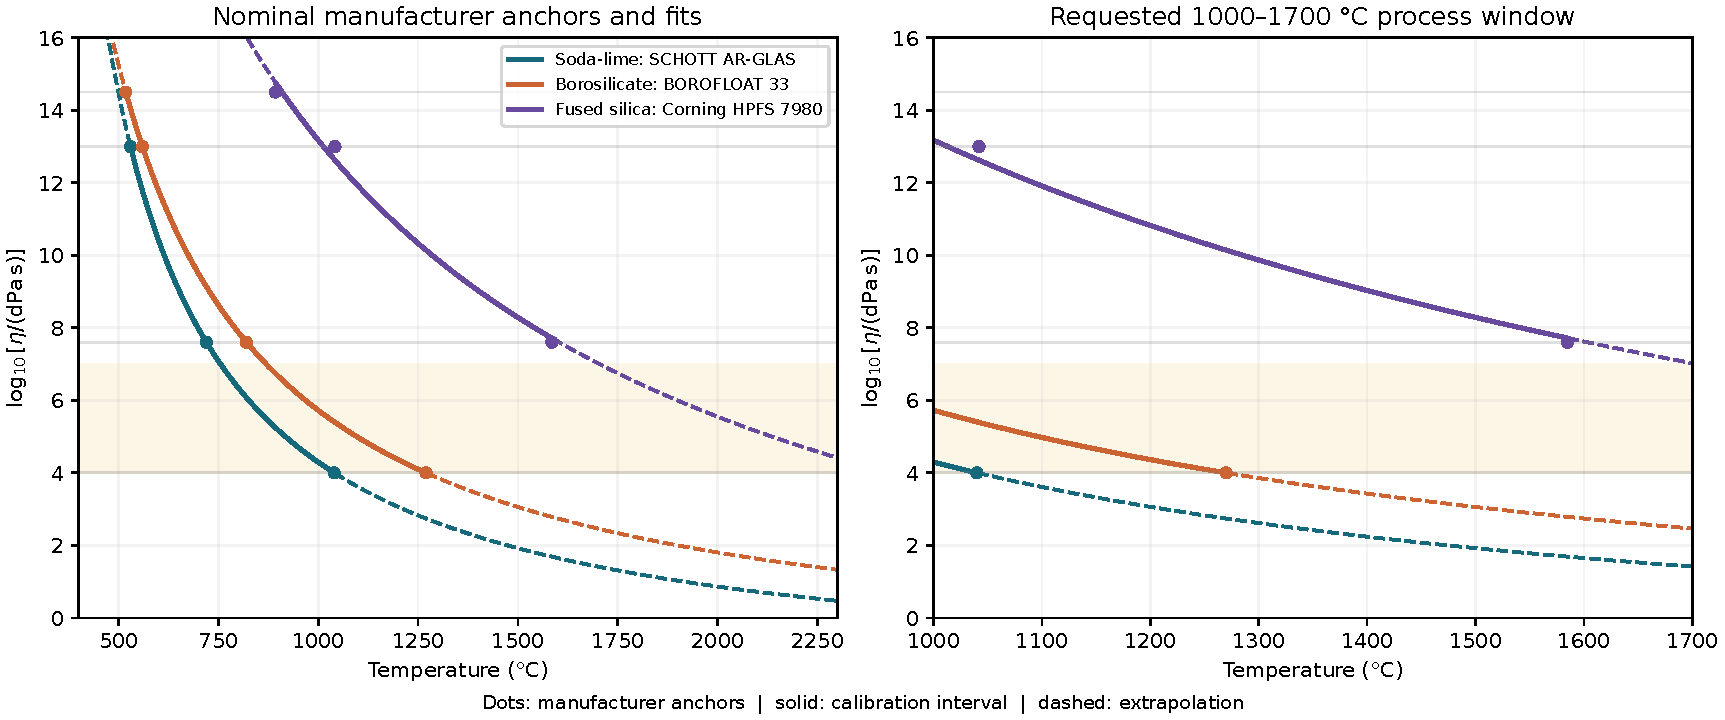
\includegraphics[width=\linewidth]{figures/viscosity_vft.pdf}
\caption{Calculated viscosity curves from nominal, composition-specific manufacturer reference points. Solid segments lie between the lowest and highest fitting anchors; dashed segments are extrapolation. The shaded $10^4$--$10^7$ dPa\,s band is a descriptive working band for comparison, not a validated universal printing window. HPFS uses the approximate constrained model described in the text.}
\label{fig:vft}\end{figure}

\begin{table}[htbp]\centering\small
\caption*{Temperatures ($^{\circ}$C) obtained by inversion of the fitted curves, deliberately distinguished from reported manufacturer points. Columns correspond to $y=14.5$, 13, 7.6, and 4. The AR-GLAS strain estimate and silica working estimate are extrapolations; the silica softening estimate slightly exceeds its calibration interval.}
\begin{tabular}{lrrrr}\toprule Material & Strain & Annealing & Softening & Working \\ \midrule
AR-GLAS & 499.4 & 530.0 & 720.0 & 1040.0 \\
BOROFLOAT 33 & 518.2 & 559.7 & 820.4 & 1269.6 \\
HPFS 7980 (approx.) & 909.5 & 1012.9 & 1603.3 & 2430.8 \\
\bottomrule\end{tabular}

\end{table}

The computed HPFS working point near 2431~$^{\circ}$C is far outside the fitted data and should be treated only as an illustration of extrapolation risk. It is not a process recommendation: evaporation, optical absorption, and equipment/material limits require separate treatment. Even the 1000--1700~$^{\circ}$C plot contains substantial extrapolation for AR-GLAS. Publishing a smooth curve does not establish its validity throughout its axis range.

\begin{figure}[htbp]\centering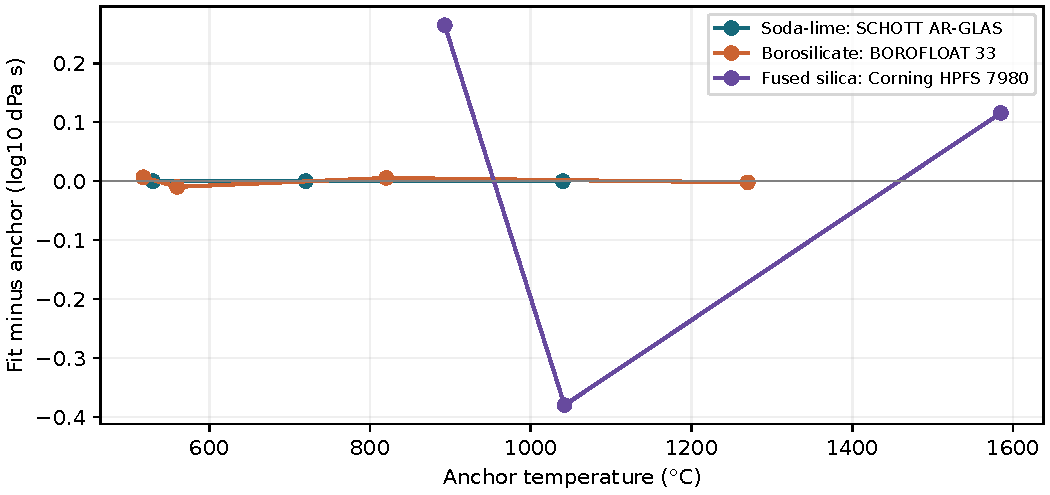
\includegraphics[width=.77\linewidth]{figures/viscosity_residuals.pdf}
\caption{Residuals reveal the approximation that a visually smooth curve can hide. The silica model is least suitable for selecting annealing setpoints. Manufacturer reference points should be retained as reported rather than silently replaced with fitted values.}
\end{figure}

\subsection{Flow, capillarity, and a worked scaling example}
For a cord radius $r$, speed $U$, density $\rho$, surface tension $\gamma$, and dynamic viscosity $\eta$, useful ratios are
\begin{equation}
 \mathrm{Re}_d=\frac{2\rho Ur}{\eta},\quad
 \mathrm{Ca}=\frac{\eta U}{\gamma},\quad
 \mathrm{Bo}_r=\frac{\rho gr^2}{\gamma},\quad
 \mathrm{Oh}_r=\frac{\eta}{\sqrt{\rho\gamma r}}.
\end{equation}
The subscripts explicitly identify the length convention; radius-based and diameter-based definitions differ. Very small Reynolds number does not mean that gravity or surface tension is negligible. It means that inertia is small relative to viscous stresses under the assumed scale.

Consider a hypothetical isothermal cylindrical nozzle with radius 5 mm, length 10 mm, melt head 0.2 m, $\rho=2500$ kg/m$^3$, $\eta=1000$ Pa\,s, and assumed $\gamma=0.3$ N/m. These are scenario inputs, not a commercial specification. Equation~\ref{eq:nozzleflow} predicts a pressure of 4905 Pa, $Q=1.204\times10^{-7}$ m$^3$/s, and 1.083 kg/h. The mean nozzle speed is 1.533 mm/s. Using that speed gives $\mathrm{Re}_d=3.83\times10^{-5}$, $\mathrm{Ca}=5.11$, $\mathrm{Bo}_r=2.04$, and $\mathrm{Oh}_r=516$. This low-inertia example is sensitive to viscosity and radius; its short nozzle also makes entrance effects a material omission. It does not predict actual accepted-part throughput.

\begin{figure}[htbp]\centering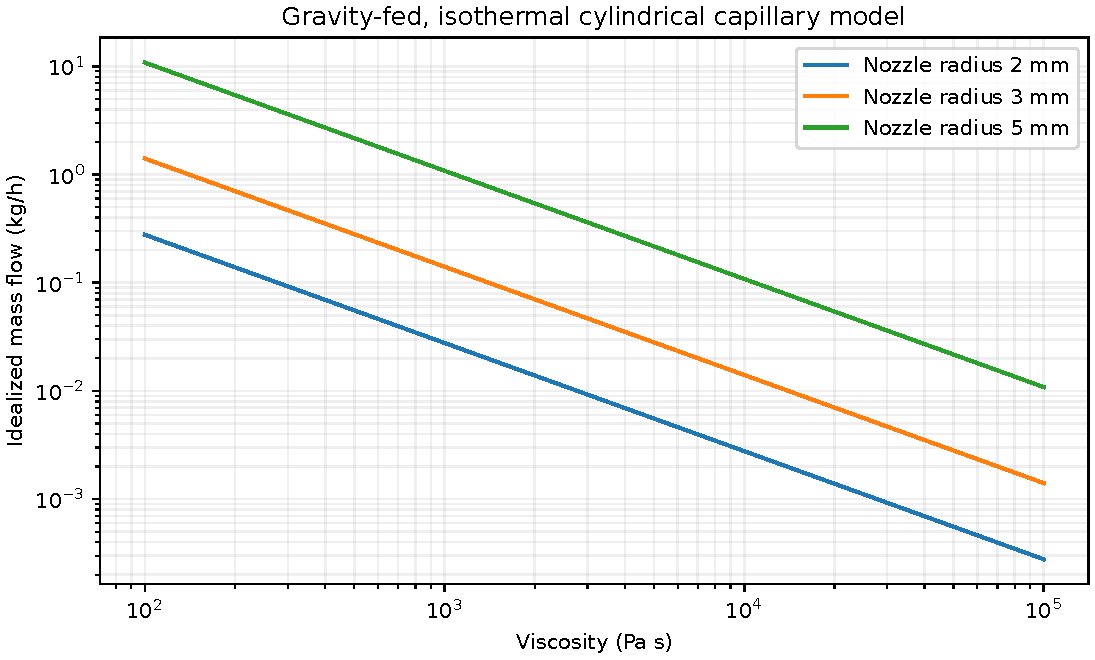
\includegraphics[width=.83\linewidth]{figures/flow_sensitivity.pdf}
\caption{Scenario calculation for a 0.2 m head, 10 mm bore length, and assumed constant density. The $r^4/\eta$ dependence explains why thermal drift and nozzle wear are important. No measured machine performance is plotted.}
\end{figure}

The local viscosity sensitivity follows directly from the fit:
\begin{equation}
 \frac{\mathrm{d}\ln\eta}{\mathrm{d}T}=-\ln(10)\frac{B}{(T-T_0)^2},\qquad
 \frac{\mathrm{d}\ln Q}{\mathrm{d}T}\simeq-\frac{\mathrm{d}\ln\eta}{\mathrm{d}T}.
\end{equation}
The second relation holds only when the other capillary-model inputs remain fixed. It motivates temperature feedback without implying that a heater command controls glass temperature instantaneously.

\subsection{Instability, slumping, and interlayer contact}
For an ideal inviscid free cylindrical jet in a dynamically negligible exterior fluid, the fastest growing axisymmetric capillary mode has wavelength approximately $9.02r=4.51d$. That familiar Rayleigh result is not a universal optimum for a viscous glass bead contacting a substrate. Viscosity contrast, cooling, stretching, finite length, contact angle, and the receiving surface change the instability problem; Tomotika's viscous-thread treatment illustrates the importance of the surrounding fluid.\cite{phys_rayleigh,phys_tomotika}

The viscous capillary scale $t_\gamma\sim\eta r/\gamma$ is about 16.7 s for the preceding scenario. A gravitational deformation scale $t_g\sim\eta/(\rho gH)$ is about 0.41 s for an assumed unsupported height $H=0.1$ m. These order-of-magnitude times refer to a material that remains at the selected viscosity. A rapidly cooling, attached bead violates that assumption, and neither value is an observed failure time. They show why shape arrest and bonding must be controlled together.

Surface-tension gradients can impose tangential stresses, $\eta\,\partial u_t/\partial n\sim\partial\gamma/\partial s$. Temperature and composition variations can therefore drive Marangoni flow even when bulk inertia is small. Quantifying it requires the actual derivative of surface tension and local thermal field; a generic sign or magnitude is not assigned here. Similarly, capillary neck growth between adjacent beads is only one contribution to adhesion. Contact area, surface contamination, and the time-temperature history must accompany any comparison of interlayer strength.

\subsection{Thermal scales and materials outside the fitted set}
Using BOROFLOAT's reference $k=1.2$ W/(m K) at 90~$^{\circ}$C, $c_p=830$ J/(kg K) over 20--100~$^{\circ}$C, and nominal density 2230 kg/m$^3$ gives an approximate low-temperature diffusivity $a\approx6.48\times10^{-7}$ m$^2$/s. Characteristic diffusion times $L^2/a$ are approximately 39 s at $L=5$ mm and 617 s at 20 mm. These are scaling calculations using low-temperature reference properties, not high-temperature annealing schedules. Radiation, temperature-dependent properties, and boundary conditions become significant in a real print.\cite{phys_boro}

Aluminosilicates add a broad composition space with varying modifiers, liquidus behavior, and viscosity. No single aluminosilicate curve is defensibly inferred from the three products above. A useful extension would specify a grade and obtain measured viscosity, expansion, crystallization kinetics, and compatible wet-contact materials before fitting. This explicit gap is preferable to assigning plausible-looking coefficients to an unspecified composition.
